\documentclass[18pt]{beamer}
\usepackage[utf8]{inputenc} % for the umlauts

\beamertemplatenavigationsymbolsempty
%% SLIDE FORMAT

% use 'beamerthemekit' for standard 4:3 ratio
% for widescreen slides (16:9), use 'beamerthemekitwide'

\usepackage{templates/beamerthemekit}
% \usepackage{templates/beamerthemekitwide}

\setcounter{tocdepth}{1}

%% TITLE PICTURE

% if a custom picture is to be used on the title page, copy it into the 'logos'
% directory, in the line below, replace 'mypicture' with the 
% filename (without extension) and uncomment the following line
% (picture proportions: 63 : 20 for standard, 169 : 40 for wide
% *.eps format if you use latex+dvips+ps2pdf, 
% *.jpg/*.png/*.pdf if you use pdflatex)

%\titleimage{mypicture}

%% TikZ INTEGRATION

% use these packages for PCM symbols and UML classes
% \usepackage{templates/tikzkit}
% \usepackage{templates/tikzuml}

% the presentation starts here

\usepackage[absolute,overlay]{textpos}
%\usepackage[texcoord,grid,gridunit=mm,gridcolor=red, subgridcolor=green]{eso-pic}

\title[SWT1]{Softwaretechnik 1 - 0. Tutorium}
\subtitle{Tutorium 03}
\author{Felix Bachmann}

\institute{KIT - Institut für Programmstrukturen und Datenorganisation (IPD)}

% Bibliography

\usepackage[citestyle=authoryear,bibstyle=numeric,hyperref,backend=biber]{biblatex}
\addbibresource{templates/example.bib}
\bibhang1em

\begin{document}

% change the following line to "ngerman" for German style date and logos
\selectlanguage{ngerman}

%title page
\begin{frame}
\titlepage
\end{frame}

%table of contents
\begin{frame}{Themenübersicht}
\tableofcontents
\end{frame}

\section{Organisatorisches}
	\subsection{Vorstellung}
		\begin{frame}
			\frametitle{Das bin ich}
			\begin{itemize}
				\item Felix Bachmann
				\item Infostudent im 4. Semester
				\item erstes Tutorium
				\item E-Post-Adresse: felix.bachmann@ewetel.net
			\end{itemize}
		\end{frame}
		\begin{frame}
			\frametitle{\dots und ihr?}
			\begin{itemize}
				\item Name
				\item Studiengang und Semester
				\item erlernte Programmiersprachen, Lieblingsprogrammiersprache
				\item Erfahrung mit Git/Maven oder ähnlichen Tools?
				\item Von dem Tutorium erwarte ich\dots
			\end{itemize}
		\end{frame}
		
	\subsection{Regeln}
		\begin{frame}
			\frametitle{Verhalten im Tutorium}
			\begin{block}{cool}
				\begin{itemize}
					\item \textbf{mitdenken}
					\item \textbf{Fragen stellen}
					\item \textbf{Fragen beantworten}
					\item essen \& trinken
					\item gehen
					\item schlafen
				\end{itemize}
			\end{block}
			\pause
			\begin{block}{!cool}
				\begin{itemize}
					\item laut sein
					\item stören
					\item andere ablenken
				\end{itemize}
			\end{block}
		\end{frame}
		
	\subsection{Übungs- und Tutoriumsbetrieb}
		\begin{frame}
			\frametitle{Übungsbetrieb}
			\begin{itemize}
				\item Bestehen des Scheins Voraussetzung zum Bestehen des Moduls
				\item neue Übungsblätter ungefähr alle 2 Wochen $\implies$ 1+6 Blätter
				\item ab 50\% der Punkte habt ihr sicher bestanden
				\item Besprechung der Musterlösung
				\pause
				\item Abgaben
					\begin{itemize}
						\item Theorieaufgaben (handschriftlich und leserlich!) + Deckblatt im 3.Stock
						\item Programmieraufgaben auf http://lez.ipd.kit.edu 
						\item Plagiate können teuer werden
						\item Deadlines sind hart!
						\item keine Abgabe per Mail!
					\end{itemize}
			\end{itemize}
		\end{frame}
		
		\begin{frame}
			\frametitle{Tutoriumsbetrieb}
			\begin{itemize}
				\item Wann?: ab dem 15.05 14-tägig 
				\item Wo?: Raum -107
				\item Was?: 
					\begin{itemize}
						\item Wiederholung des VL-Stoffs
						\item "'Rechnen"' von Aufgaben (Altklausuren)
						\item ggf. Tipps für die Übungsblätter
					\end{itemize}
				\item Folien gibt's im Ilias und auf \url{www.github.com/malluce/swt1-tut}
				\item Fragen stellen !!
			\end{itemize}
		\end{frame}
		
	\subsection{Fragen}
		\begin{frame}
			\frametitle{Fragen zu Übung(sblättern), Vorlesung}
			erst im Forum, auf Google oder Stackoverflow nachschauen, dann
				\begin{itemize}
					\item neuen Forum-Thread anlegen
					\item falls nicht öffentlich postbar: Mail an mich oder swt1@ipd.kit.edu (nur im Notfall)
				\end{itemize}
		\end{frame}
		
	\subsection{Warum Softwaretechnik?}
		\begin{frame}
			\frametitle{Warum Softwaretechnik?}
			\begin{itemize}
				\item Programmieren $\implies$ SWT1 $\implies$ PSE
				\item den Hacker strukturieren 
				\item den Umgang mit wichtigen Tools (insb. Build-Management-Tools, Versionsverwaltung) erlernen
			\end{itemize}
		\end{frame}
		
\section{Vorbereitungsblatt}
	\subsection{Bisher}
	\begin{frame}
		\frametitle{Was ihr bisher getan haben solltet..}
		Installation von:
		\begin{itemize}
			\item Eclipse (incl. CheckStyle und EclEmma)
		\end{itemize}
		Überblick über:
		\begin{itemize}
			\item Maven
			\item Git
		\end{itemize}
		\begin{alertblock}{Tut euch den Gefallen}
			\begin{itemize}
				\item Installiert Git manuell!
			\end{itemize}
		\end{alertblock}
		Probleme mit der Installation? $\implies$ kommt nach dem Tut nach vorne
	\end{frame}
		
	\subsection{Feedback Vorbereitungsblatt}	
	\begin{frame}
		\frametitle{Feedback Vorbereitungsblatt}
		%TODO Feedback für Abgaben, Statistik?
	\end{frame}
			
\section{JUnit4}	
	\subsection{JUnit4}
	\begin{frame}
		\frametitle{JUnit4 - Überblick}
		\begin{textblock*}{20mm}(60mm,5mm)
			
\includegraphics[width=30mm, scale=0.8]{./pics/tut0/junit-logo.png}
		\end{textblock*}
		\begin{itemize}
			\item Unittest-Tool für Java-Klassen
			\item über die pom.xml mit scope "'test"' einbinden
			\item Nur öffentliche Methoden testen
			\item Konventionen:
			 \begin{itemize}
			 		\item Für Klasse Hallo Testklasse HalloTest schreiben
			 		\item Methode hallo(Object o) wird z.B. durch die Methode testHalloWithNull() getestet
			 \end{itemize}
		\end{itemize}
	\end{frame}	
	
	\subsection{JUnit4 - Testklasse}
	\begin{frame}
		\frametitle{JUnit4 - Aufbau einer Testklasse}
		Methoden können mit Annotationen (@XYZ) versehen werden \linebreak
		Aufbau:
		\begin{itemize}
			\item @BeforeClass (wird als erstes einmal ausgeführt)
			\pause
			\item @Before (wird vor jeder Test-Methode einmal ausgeführt)
			\pause
			\item @Test (vergleichen erwartetes und reales Ergebnis, schlagen ggf. fehl, Ausführung in beliebiger Reihenfolge)
			\pause
			\item @After (wird nach jeder Test-Methode einmal ausgeführt)
			\pause
			\item @AfterClass (wird am ende einmal ausgeführt)
		\end{itemize}
	\end{frame}
	
	\subsection{JUnit4 - Assert}
	\begin{frame}
		\frametitle{JUnit4 - Assert}
		\begin{itemize}
			\item org.junit.Assert bietet diverse Methoden, um Ergebnis mit Erwartung abzugleichen 
			\item zu jeder Methode kann als erstes Argument ein String mitgegeben werden (wird bei Fehlschlag angezeigt) \linebreak
		\end{itemize}
		Beispiele:
		\begin{itemize}
			\item assertArrayEquals(int[] expected, int[] actual)
			\item assertNotNull(Object obj)
			\item assertSame(Object expected, Object actual)
		\end{itemize}
	\end{frame}
	
	\subsection{JUnit4 - eine Testmethode}
	\begin{frame}
		\frametitle{JUnit4 - eine Testmethode}
		\begin{block}{Zu testende Methode in der Klasse Hallo}
				public static int add(int a, int b) \{ \linebreak
					 return a + b; \linebreak
				      \}	
		\end{block} 
		\begin{block}{Testmethode in der Klasse HalloTest}
			@Test\linebreak
			public void testAdd() \{ \linebreak
				Assert.assertEquals(7, Hallo.add(5, 2)); \linebreak
			\}
		\end{block}
		(mehr Beispiele später)
	\end{frame}
	
	\subsection{JUnit4 - Fragen}
	\begin{frame}
		\frametitle{JUnit4 - Quiz}
		\begin{block}{A, B oder C?}
			Welche Annotation führt dazu, dass die annotierte Methode nach jeder mit @Test versehenen Methode einmal ausgeführt wird?
			\begin{itemize}
				\item A: @Ignore
				\item B: @After
				\item C: @AfterClass
			\end{itemize}
		\end{block}
		\pause
		\begin{block}{Wahr oder falsch?}
			Die mit @Test versehenen Methoden werden in der Reihenfolge ausgeführt, in der sie im Quellcode stehen.
		\end{block}
		\pause
		\begin{block}{Wahr oder falsch?}
			Um Ergebnisse von Methodenaufrufen mit dem erwarteten Ergebnis abzugleichen, benutzt man Methoden aus junit.framework.Assert.
		\end{block}
	\end{frame}
		
\section{Maven}

	\subsection{Maven - Überblick}
	\begin{frame}
		\frametitle{Maven - Überblick}
		\begin{itemize}
			\begin{textblock*}{20mm}(60mm,5mm)
				
\includegraphics[width=40mm, scale=1.0]{./pics/tut0/Maven_logo.png}
			\end{textblock*}
			\item Maven ist Jiddisch und heißt "'Sammler des Wissens"'
			\item Build-Management-Tool (Automatisierung von möglichst vielen Schritten)
			\item Maven ist in jeder Eclipse-Installation integriert \linebreak $\implies$ keine manuelle Installation nötig
			\item Aufgaben von Maven
				\begin{itemize}
					\item Strukturierung (durch vorgegebene Verzeichnisstruktur)
					\item Kompilieren
					\item Testen
					\item Verwalten von Abhängigkeiten
					\item Verpacken
				\end{itemize}
		\end{itemize}
	\end{frame}
	
	\subsection{Maven - Überblick}
	\begin{frame}
		\frametitle{Maven - Überblick}
		Verzeichnisstruktur:
		\begin{itemize}
			\item src
			\begin{itemize}
				\item main
				\begin{itemize}
					\item java
					\item resources
				\end{itemize}
				\item test
				\begin{itemize}
					\item java
					\item resources
				\end{itemize}
			\end{itemize}
			\item target
			\begin{itemize}
				\item classes
				\item test-classes
				\item *.jar / *.war / *.zip \dots
				\item \dots
			\end{itemize}
			\item pom.xml
		\end{itemize}
	\end{frame}
	
	\subsection{Maven - pom.xml}
	\begin{frame}
		\frametitle{Maven -pom.xml}
		\begin{itemize}
			\item pom steht für "'Project Object Model"'
			\item konfiguriert euer Maven Projekt im XML-Format (gefüllt durch default-Werte)
			\begin{itemize}
				\item Wo sucht Maven Tests?
				\item Wohin speichert Maven Build-Dateien?
				\item In welches Format soll das Projekt verpackt werden?
				\item \dots
			\end{itemize}
			\item Eclipse-Plugin bietet GUI
		\end{itemize}
	\end{frame}
	
	\subsection{Maven - Wichtige Befehle}
	\begin{frame}
		\frametitle{Maven - Überblick}
		\begin{block}{Wichtige Befehle}
			\begin{tabular}{ll}
				\texttt{mvn compile} & kompiliert Quelltexte zu .class-Dateien \\
				\texttt{mvn test} & kompiliert Test-Quelldateien zu .class-Dateien, \\ & führt Tests aus und zeigt Ergebnisse an \\
				\texttt{mvn package} & verpackt euer Projekt in eine Datei (.war/.jar/.zip) \\ 
				\texttt{mvn clear} & leert euren target-Ordner \\
			\end{tabular}
		\end{block}
	\end{frame}
	
	\subsection{Maven - Debugging}
	\begin{frame}
		\frametitle{Maven - Fehler finden}
		Lösungsansätze:
		\begin{itemize}
			\item Rechtsklick auf Projekt $\implies$ Maven $\implies$ Update Maven Project $\implies$ Haken bei "'Force Update..." 
			\begin{itemize}
				\item Synchronisiert pom.xml mit Projekt, aktualisiert Abhängigkeiten
			\end{itemize}
			\item mvn clean
			\begin{itemize}
				\item vielleicht war der target-Ordner verschmutzt
			\end{itemize}
			\item C:/Users/MeinName/.m2/ löschen und mvn compile (oder mvn package) ausführen
			\begin{itemize}
				\item löscht alle Dependencies und lädt sie neu runter (ab und zu lädt man leider korrupte Dateien runter oder Dateien fehlen)
			\end{itemize}
		\end{itemize}
	\end{frame}
	
	\subsection{Maven - Quiz}
	\begin{frame}
		\frametitle{Maven - Quiz}
		\begin{block}{A, B, C oder D?}
			Welcher Maven-Befehl kompiliert die Testklassen?
			\begin{itemize}
				\item A: mvn compile
				\item B: mvn package
				\item C: mvn test
				\item D: mvn test-compile
			\end{itemize}
		\end{block}
		\pause
		\begin{block}{Wahr oder falsch?}
			Damit Maven funktioniert, muss die komplette pom.xml manuell ausgefüllt werden. 
		\end{block}
	\end{frame}


\section{Git}
	\subsection{Warum Versionsverwaltung?}
	\begin{frame}
		\frametitle{Warum Versionsverwaltung?}
		\begin{figure}
			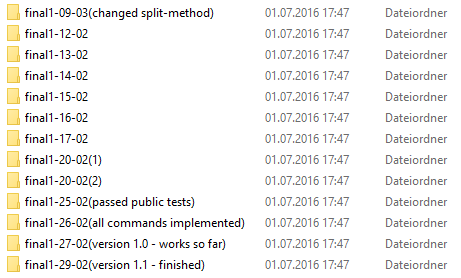
\includegraphics[scale=0.7]{./pics/tut0/bad-version-management.png}
			\linebreak
			\centering 			So nicht!
		\end{figure}	
	\end{frame}
	
	\subsection{Git - Überblick}
	\begin{frame}
		\frametitle{Git - Überblick}
		\begin{textblock*}{20mm}(60mm,5mm)
			
\includegraphics[width=30mm, scale=0.8]{./pics/tut0/Git-logo.png}
		\end{textblock*}
		\begin{itemize}
			\item git ist Englisch, bedeutet Schwachkopf, Penner oder Nudelauge (?)
			\item dezentrales Versionsverwaltungssystem
			\item wichtig! (universell)
		\end{itemize}
	\end{frame}
	
	\begin{frame}
		\frametitle{Umgang mit der Kommandozeile (cmd)}
		Nötig?\linebreak
		\begin{block}{Wichtige Befehle - Navigation}
			\begin{tabular}{ll}
				\texttt{cd test} &  Wechselt in das Verzeichnis test.\\
				\texttt{dir bzw. ls} &  Zeigt Inhalt des aktuellen Ordners an.\\
				\texttt{.} & = aktuelles Verzeichnis\\ 
				\texttt{..} & = übergeordnetes Verzeichnis\\
			\end{tabular}
		\end{block}
		
		\begin{alertblock}{Hacks}
			\begin{itemize}
				\item Mit den Pfeiltasten können bereits eingegebene Befehle durchgescrollt werden.
				\item Tabulator = Autovervollständigung
			\end{itemize}
		\end{alertblock}
		
	\end{frame}
	
	\subsection{Git - Befehle}
	\begin{frame}
		\frametitle{Git - Überblick}
		\begin{block}{Wichtige Befehle}
			\begin{tabular}{ll}
				\texttt{git init} &  Initialisiert ein leeres Git-Repo.\\
				\texttt{git log} &  Zeigt alle vergangenen Commits.\\
				\texttt{git status} &  Zeigt den Status der Dateien im Repo.\\
				\texttt{git checkout} & \begin{small}
					Lässt HEAD zwischen Commits springen. 
				\end{small}\\
				\texttt{git add} &  Fügt Datei(en) zur Staging Area hinzu.\\
				\texttt{git commit -m "message"} &  Erzeugt einen Commit.\\ 
			\end{tabular}
		\end{block}
		\centering 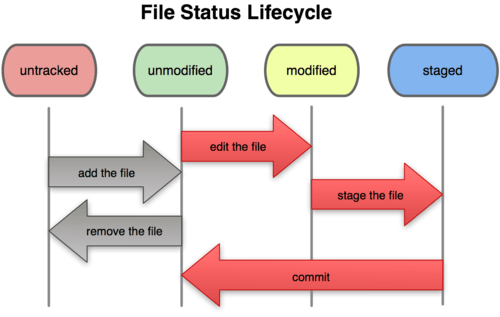
\includegraphics[width=60mm, scale=1.5]{./pics/tut0/git-file-lifecycle.png}
	\end{frame}

	\subsection{Git - .gitignore}
	\begin{frame}
		\frametitle{Git - .gitignore}
		\begin{itemize}
			\item Datei, die Namen von Pfaden/ Dateien enthält, die von git ignoriert werden sollen (z.B IDE-spezifisches)
			\item Beispiele: 
			\begin{itemize}
				\item target/
				\item *.java
				\item dis.like
			\end{itemize}
			\item \# dient als Kommentar-Zeichen
		\end{itemize}
	\end{frame}
		
\section{Live-Demo}		
	\subsection{Live-Demo}
	\begin{frame}
		\centering Live-Demo
	\end{frame}
		
\section{Tipps}
	\subsection{Tipps}
	\begin{frame}
		\frametitle{Tipps - 1. Übungsblatt}
		\begin{small}
			\begin{exampleblock}{Aufgabe 1: Altsoftware vorbereiten}
				\begin{itemize}
					\item löchriges Kochrezept für Umgang mit Maven, Git, Checkstyle - da müsst ihr durch
					\item Google ist euer Freund (meistens)
				\end{itemize}
			\end{exampleblock}
			\pause
			\begin{exampleblock}{Aufgabe 2: Modultests}
				\begin{itemize}
					\item Aufgaben zum Testen mit JUnit4
					\item Ordner sollen erstellt werden, wenn sie nicht existieren
					\item Asserts benutzen !
				\end{itemize}
			\end{exampleblock}
			\pause
			\begin{exampleblock}{Aufgabe 3: Testüberdeckung}
				\begin{itemize}
					\item Mockito klingt komplizierter als es ist (schaut mal auf \url{https://www.javacodegeeks.com/2012/05/mocks-and-stubs-understanding-test.html})
				\end{itemize}
			\end{exampleblock}
		\end{small}
	\end{frame}
	
	\subsection{Abgabe}
	\begin{frame}
		\frametitle{Denkt dran!}
		\begin{alertblock}{Abgabe}
			\begin{itemize}
				\item in der LEZ bis zum 10.05, 12:00
				\item falls ihr ein Feedback wollt, werft das Deckblatt ein
			\end{itemize}
		\end{alertblock}
	\end{frame}
		
	\begin{frame}
		\frametitle{Bis dann! (dann=15.05.17)}
		\centering
		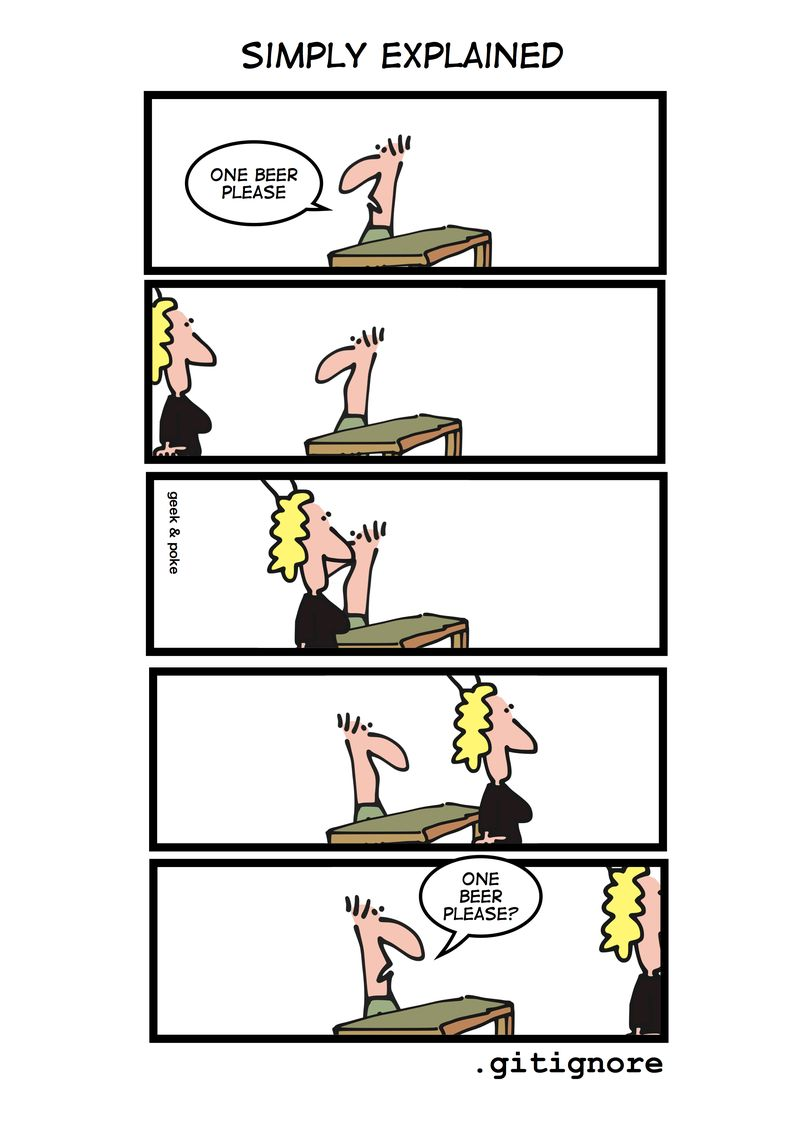
\includegraphics[height=0.85\textheight]{./comics/geek_and_poke_gitignore.jpg}
		\tiny\url{geek-and-poke.com/geekandpoke/2012/11/7/simply-explained.html}
	\end{frame}

\end{document}
